% !TEX root = ../thesis.tex

\chapter{Príručka pre správcu}

% \section*{Karel's Primitives}

% \begin{itemize}
%     \item \verb|void movek()| - Moves \textit{Karel} one intersection forward.
%     \item \verb|void turn_left()| - Pivots \textit{Karel} $90$ degrees left.
%     \item \verb|void pick_beeper()| - Takes a beeper from the current intersection and puts it in the beeper bag.
%     \item \verb|void put_beeper()| - Takes a beeper from the beeper bag and puts it at the current intersection.
%     \item \verb|void turn_on(char* path)| - Turns \textit{Karel} on.
%     \item \verb|void turn_off()| - Turns \textit{Karel} off.
% \end{itemize}


% \section*{Karel's Sensors}

% \begin{itemize}
%     \item \verb|int front_is_clear()| - Returns \texttt{1} if there is no wall directly in front of \textit{Karel}. \texttt{0} if there is.
%     \item \verb|int right_is_clear()| - Returns \texttt{1} if there is no wall immediately to \textit{Karel}'s right. \texttt{0} if there is.
%     \item \verb|int beepers_present()| - Returns \texttt{1} if \textit{Karel} is standing at an intersection that has a beeper. \texttt{0} otherwise.
%     \item \verb|int facing_north()| - Returns \texttt{1} if \textit{Karel} is facing north. \texttt{0} otherwise.
%     \item \verb|int beepers_in_bag()| - Returns \texttt{1} if there is at least one beeper in \textit{Karel}'s beeper bag. \texttt{0} if the beeper bag is empty.
% \end{itemize}


% \section*{Misc Functions}

% \begin{itemize}
%     \item \verb|void set_step_delay(int)| - Sets delay of one \textit{Karel}'s step in miliseconds.
%     \item \verb|loop(int)| - Repeats \textit{Karel}'s instruction in a loop.
% \end{itemize}


Táto príručka je určená pre správcu crawlera. Rozoberieme si ako crawler inicializovať, monitorovať jeho beh. \todo{doplnenie}

Sme názoru, že dobre napísaný kód je seba dokumentujúc. Preto popíšeme iba princípy a a kroky potrebné pre vykonanie bežných úkonov. 

\section{Príprava prostredia}
Crawler nie je závislí na žiadnom externom systéme. Teda netreba nasadzovať databázu ani nič podobné. 

Je potrebné mať JRE (Java Runtime Environment), ale odporúčame JDK (Java Development Kit) verzie 11. 

\section{Inicializácia}
Pri inicializácii vieme crawleru poskytnúť rôzne implementácie modulov a tým ovplyvniť jeho správanie. Napríklad ak bude potrebné zmeniť ukladanie výsledkov z CSV formátu do iného, stačí implementovať novú verziu repozitára a pri inicializácii ňou naplniť CrawlerContext. Podrobný postup je znázornený na diagrame \ref{o:initChart} a ukážka kódu je na  \ref{o:initCrawl2}

Dôležitou súčasťou nastavení je aj veľkosť kroku (stepMaxSize), udávajúca počet adries spracovaných v jednom kroku. Jej zvýšením vieme zefektívniť beh programu, keďže redukujeme počet neparalelných úsekov a prístup do súborového systému. Na druhú stranu ale zvyšujeme nároky na pamäť, keďže v nej pred uložením držíme práve tento počet výsledkov extrahovania. Teda ak zvo-
líme tento parameter príliš vysoký, program môže vyčerpať pridelenú operačnú pamäť. Oproti tomu menším problémom je aj zväčšenie veľkosti stratených dát pri páde programu.

\begin{figure}[!ht]
    \centering
    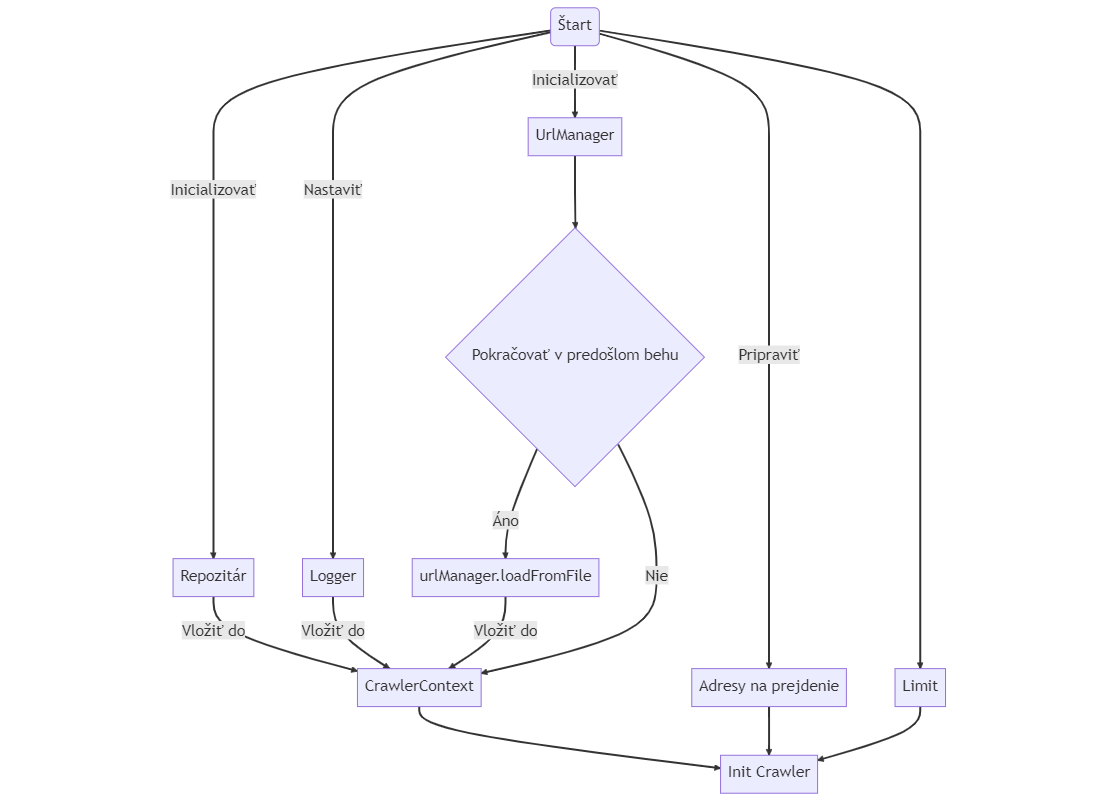
\includegraphics[width=1\textwidth]{figures/initChart.png}
    \caption{Diagram inicializácie crawlera\label{o:initChart}}
\end{figure}

\begin{figure}[!ht]
    \centering
    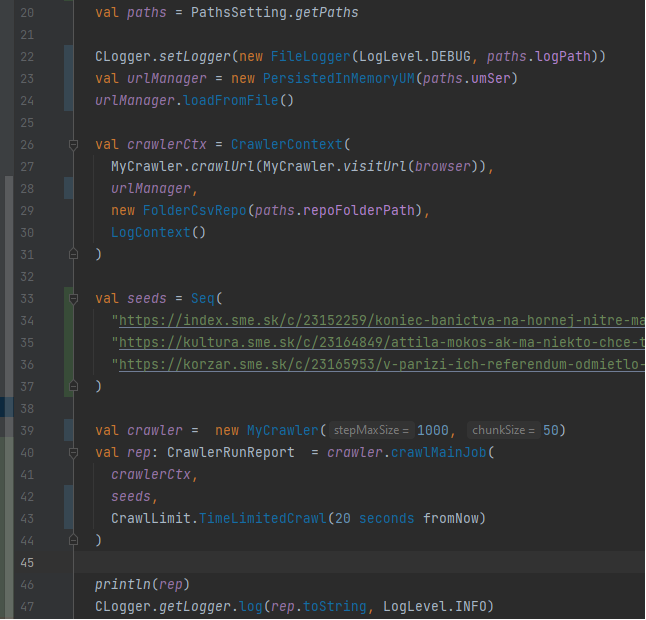
\includegraphics[width=.9\textwidth]{figures/crawlInit.png}
    \caption{Ukážková iniclializácia crawlera\label{o:initCrawl2}}
\end{figure}

\section{Vyhodnotenie štatistík}
Crawler zbiera štatistiky pomocou záznamov ukladaných do súbory. Skript XXXX \ref{nazov} ich potom spracuje a zapíše do CSV súboru. 

Odporúčame každý jeden stĺpec dať do samostatného grafu. Výsznam stĺpcov: 
\begin{itemize}
    \item \textbf{crawlT} - trvanie crawlovacej aktivity - jej plávajúci priemer má byť konštatntný - rastúci trend indikuje problém s pripojením na server zapríčinenú príliš veľkou paralelizáciou (nanosekundy)
    \item \textbf{stepT} - dĺžka jedného kroku - tiež by mala byť konštantná (milisekundy)
    \item \textbf{batchT} - trvanie získania adries na prejdenie v danom kroku (nanosekundy)
    \item \textbf{upsertT} - trvanie pridania nových adries na prejdenie - očakávame mierny lineárny nárast (nanosekundy)
    \item \textbf{upsertT} - trvanie pridania nových adries na prejdenie - očakávame mierny lineárny nárast (nanosekundy)
\end{itemize}


\section{}